\documentclass[journal]{IEEEtran}
\usepackage[a5paper, margin=10mm, onecolumn]{geometry}
\usepackage{tfrupee}
\usepackage{amsmath, amssymb, amsfonts, amsthm}
\usepackage{algorithmic}
\usepackage{graphicx}
\usepackage{textcomp}
\usepackage{xcolor}
\usepackage{txfonts}
\usepackage{listings}
\usepackage{enumitem}
\usepackage{mathtools}
\usepackage{gensymb}
\usepackage{comment}
\usepackage[breaklinks=true]{hyperref}
\usepackage{tkz-euclide} 
\usepackage{listings}
\usepackage[latin1]{inputenc}                                
\usepackage{color}                                            
\usepackage{array}                                            
\usepackage{longtable}                                       
\usepackage{calc}                                             
\usepackage{multirow}                                         
\usepackage{hhline}                                           
\usepackage{ifthen}                                           
\usepackage{lscape}
\newcommand{\myvec}[1]{\begin{pmatrix} #1 \end{pmatrix}}

\begin{document}

\bibliographystyle{IEEEtran}
\vspace{3cm}

\title{NCERT-9.7.14}
\author{EE24BTECH11042 - SRUJANA}
{\let\newpage\relax\maketitle}

\renewcommand{\thefigure}{\theenumi}
\renewcommand{\thetable}{\theenumi}
\setlength{\intextsep}{10pt} 

\numberwithin{equation}{enumi}
\numberwithin{figure}{enumi}
\renewcommand{\thetable}{\theenumi}

\textbf{QUESTION}:

Find the particular solution of the differential equation $(x+1)\frac{dy}{dx} = 2 e^{-y}-1$, given that y = 0 when x = 0

\textbf{Theoretical Solution:}

\begin{align}
    \frac{dy}{dx} &= \frac{2 e^{-y}-1}{x+1}\\
    \frac{dy}{2 e^{-y}-1} &= \frac{dx}{x+1}
\end{align}
Integrating on both sides
\begin{align}
   e^y = 2-\frac{1}{x+1} \cdot c 
\end{align}
Substitute initial conditions in 0.3
\begin{align}
    1 &= 2-1 \cdot c \implies c=0\\
    e^y &= \frac{2x+1}{x+1}
\end{align}
Final solution 
\begin{align}
   y = \ln{\left( \left| \frac{2x+1}{x-1} \right| \right)}
\end{align}
\textbf{Solution by finite differences method}

The finite difference method is used to calculate the solutions of differential equations.

\begin{align}
    \frac{dy}{dx} &= \lim_{h \to 0}\frac{f(x+h)-f(x)}{h}\\
    f(x+h) &= \frac{dy}{dx} \cdot h + f(x)\\
    y_{n+1} &= \frac{2 e^{-y_n}-1}{x_n+1} \cdot h + y_n\\
    x_{n+1} &= x_n + h 
\end{align}

Substitute the initial conditions into the differential equation to find $\frac{dy}{dx}$ at those points. 

Assume $h = 0.01$, and calculate $f(x+h)$. 

Now, use $x+h$ and $f(x+h)$ as the new initial conditions. 

Repeat this process until you have sufficient points to plot the graph. 

Connect all the points to obtain an approximate plot of the differential equation. 

This is the graphical representation of both simulation and theoretical approaches 

\begin{figure}[h!]
   \centering
   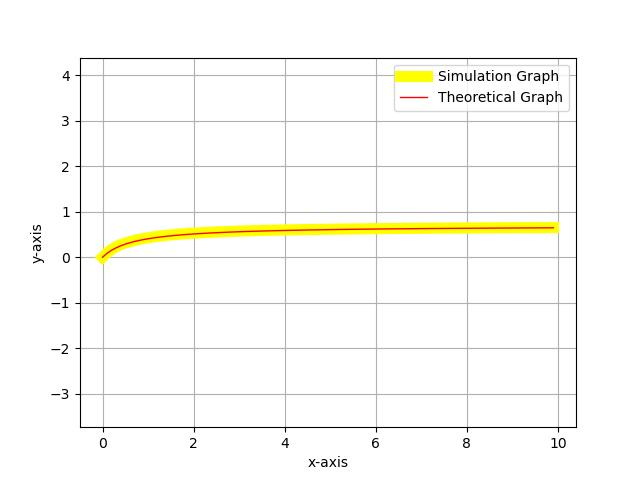
\includegraphics[width=\columnwidth]{fig/combined_fig.jpg}
\end{figure}

\end{document}

